\chapter{Standards and Regulations}
\label{cha:standards}

Until the so-called third industrial age, or Industry 3.0, cybersecurity had minimal impact on manufacturing. Industrial machinery wasn't necessarily connected to the internet or each other, making external risks unlikely. However, with the dawn of Industry 4.0, smart machinery and smart factories have become vital for the smooth operation of production departments, placing cybersecurity at the forefront of concern.

Cybersecurity involves protecting systems, networks, and programs from digital attacks. Given the critical nature of the topic and the attention it demands, companies are embarking on paths to elevate their awareness of cyberattacks, adopting internal policies, or even pursuing specific certifications in cybersecurity. Concurrently, national and international legislators have introduced new legislative measures imposing new obligations on certain entities in relation to cybersecurity.

Let's now consider the most recent legislative measures on cybersecurity and the related certifications that manufacturing industries must take into account.\\
Certifications provide a guarantee of product and company security. The main certifications currently considered include:
\begin{itemize}
  \item \textbf{IEC 62443}: This series of international standards is renowned for enhancing the security of industrial control systems, setting forth fundamental prerequisites to shield industrial systems from cyber threats;
  \item \textbf{ISO/IEC 27001 (2022)}: This certification covers various aspects, including security policy, human resource security, physical and environmental security, communications management, and regulatory compliance;
\end{itemize}

There are then several laws and regulations that address under various profiles the issue of cybersecurity among them it is worth noting:~\cite{cybersecurity-standards-regulations-compliance}
\begin{itemize}
  \item \textbf{Cyber Resilient Act (CRA)}\footnote{\url{https://eur-lex.europa.eu/legal-content/EN/TXT/?uri=celex:52022PC0454}}: While still pending final approval by the European Institutions, the Cyber Resilient Act seeks to enhance the resilience of the European digital market by ensuring that connected devices and digital services are equipped to withstand cyberattacks effectively. It will become effective in 2027;
  \item  \textbf{NIS Directive 2}\footnote{\url{https://eur-lex.europa.eu/legal-content/EN/TXT/?uri=CELEX:32022L2555}}: This directive outlines essential criteria that companies must adhere to in order to maintain a robust level of cybersecurity. These criteria encompass the implementation of risk analysis strategies, fortification of information system security, and effective incident management protocols. It is imperative for EU Member States to transpose this directive by October 2024, with enforcement timelines specified in the respective national transposition acts;
  \item \textbf{Italian Cybersecurity Law (June 28th, 2024 No. 90)}\footnote{\url{https://www.gazzettaufficiale.it/eli/id/2024/07/02/24G00108/sg}}: This Italian law pertains to national cybersecurity and applies to both public and private entities whose services are deemed critical. It mandates the implementation of security measures to protect critical digital infrastructures and sensitive information, including specific obligations to notify the Cybersecurity Agency of any cyber incidents;
  \item \textbf{New Machinery Regulation No. 1230/2023}\footnote{\url{https://eur-lex.europa.eu/legal-content/EN/TXT/?uri=CELEX:32023R1230}}: This regulation will replace the Machinery Directive No. 2006/42/EC, focusing on the overall safety of machinery and semi-machinery and it will become effective in 2027. It emphasizes the essential integration of cybersecurity into the design and manufacturing processes of machinery, recognizing the potential risks that cyber vulnerabilities pose to physical safety;
\end{itemize}

This chapter will provide an overview of the most relevant standards and regulations for the context of the internship's researches, focusing on the industrial sector and the required goals; in particular, we will detail more about \textit{IEC 62443}, \textit{ISO 27001} and \textit{CRA}.

\section{IEC 62443}

The IEC 62443 provides guidelines, rules and definitions specifically crafter for any Industrial Control System (ICS) and Industrial Automation and Control Systems (IACS). Compared to ISO 27001, it is more focused on the specific sector instead of being more universal and open for the interpretation depending on the company it applies on.

The market requires the IEC 62443 certification for the companies that are involved in the production of industrial devices, as it is a guarantee of the security of the product and the company itself. 

The IEC 62443 is a set of standards drafted by the \textit{Internation Electrotechnical Commission} (IEC) and it is divided into four categories:~\cite{understanding-iec-62443-parts}
\begin{enumerate}
  \item \textbf{General}: it covers topics that are common to the entire series;
  \item \textbf{Policies and procedures}: focuses on methods and processes associated with IACS security;
  \item \textbf{System}: it covers the requirements for the secure development and integration of systems;
  \item \textbf{Component}: it covers the requirements for the secure development and integration of components.
\end{enumerate}

\begin{figure}[t]
  \centering
  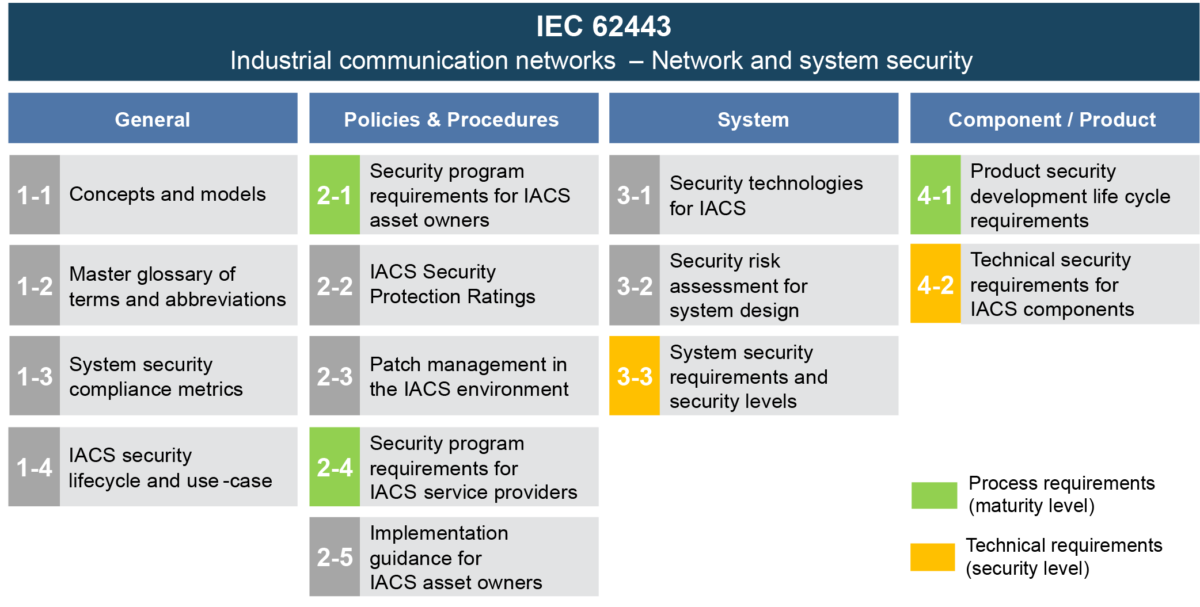
\includegraphics[width=0.9\textwidth]{chapters/03/assets/iec62443.png}
  \caption[IEC 62443 Parts and Sections. Image by Mohamed Wassef O. \protect\footnotemark]{IEC 62443 Parts and Sections. Image by Mohamed Wassef O. \protect\footnotemark}
  \label{fig:iec-62443}
\end{figure}
\footnotetext{\url{https://www.linkedin.com/pulse/power-iec-62443-safeguarding-industrial-automation-othmani-gsrde}}

Each category is divided into several subcategories, corresponding to different subjects and requirements. The IEC 62443 is a comprehensive standard that covers all the specific aspects starting from the product design up to the development.

Each subcategory, identified by the category number followed by an increasing index, contains a list of System Requirements (SR) that the company must meet to obtain the certification. 

In example, a system requirement taken from the subcategory \textit{System security requirements and security levels} (\texttt{3-3}) is the one shown in~\cref{fig:iec62443_3-3_3_9}. We are going to explain it in detail.

The SR 3.9 states the following:
\begin{mdframed}
  SR 3.9 - Protection of audit information: The control system shall protect audit information and audit tools (if present) from unauthorized access, modification and deletion.
\end{mdframed}\label{sr:3-3_3-9}

Log audit are essential for prevention and detection of cyberattacks. When something goes wrong, the log audit can help to understand what happened, when and where it happened, and who was involved. This is a fundamental requirement for the IEC 62443 certification.

For each Security Requirement listed in the documentation, the standard also describes some potential rationale and supplemental guidance to help the company to understand the requirement and how to implement it.

Each SR is made of four security levels. \\
A Security Level (SL) is a measure of the security of a system or component, which is eventually transmitted to the final client. It is a score from 1 to 4, where 1 indicates the lowest complexity of the solution we can apply to follow the requirement, and 4 indicates the highest complexity.~\cite{ixon-practical-guide-iec-62443}

It is possible to increase the score of the security level by applying more non-trivial solutions, expressed as a \textit{Requirement Enhancement}. An enhancement to increase the security level from 3 to 4 is stated in \texttt{SR 3.9 RE 1}:
\begin{mdframed}
  SR 3.9 RE 1 - Audit records on write-once media: The control system shall provide the capability to produce audit records on hardware-enforced write-once media.
\end{mdframed}\label{sr:3-3_3-9_re1}

We would like to note that not every SR has exactly four RE; instead, it could be that there are less solutions in order to increase its score. For instance, this is the case for the SR 3.9, which has only one RE and the minimum applicable security level is the level 2, as shown in~\cref{fig:iec-62443_3-3_3_9}.

\begin{figure}[t]
  \centering
  \fbox{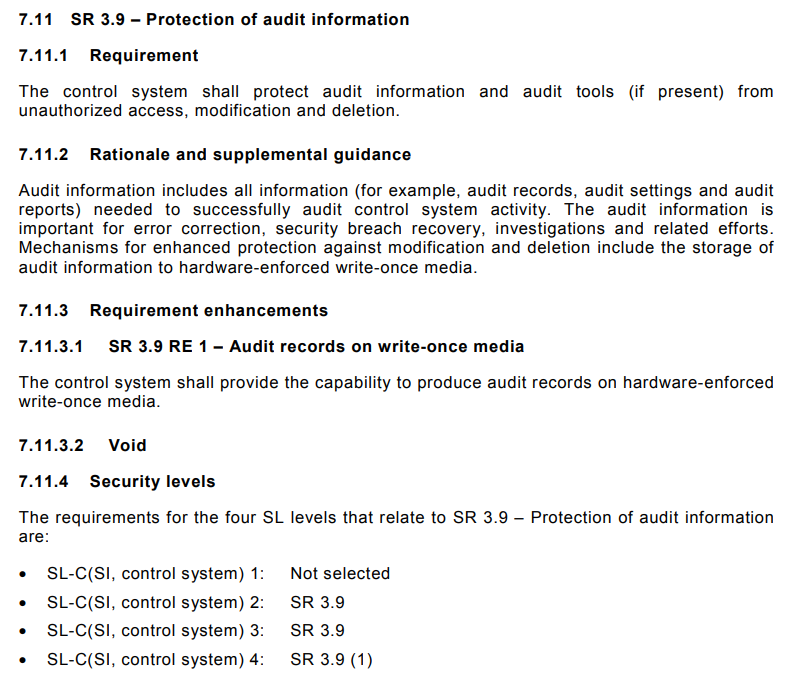
\includegraphics[width=1.0\textwidth]{chapters/03/assets/iec62443_3-3_3_9.png}}
  \caption[Snapshot of a System Requirement]{Snapshot of a System Requirement}
  \label{fig:iec62443_3-3_3_9}
\end{figure}

Moreover, sometimes the highest security level is not always the best solution or the most suitable for the company. Therefore, it is essential to evaluate the cost and the benefits of the solution before applying it.


In the context of the company we are working with and the internship project we are involved in, because we are directly at the level of product design and component development and deployment, the relevant subcategories we are focusing on are \texttt{3-3}, \texttt{4-1} and \texttt{4-2}, respectively named \textit{System security requirements and security levels}, \textit{Product security development life cycle requirements} and \textit{Technical security requirements for IACS components}.

At the system level, \texttt{IEC 62443-3-3} introduces security levels and corresponding requirements, offering a scalable framework to protect industrial systems. This part enables organizations to customize their security measures based on specific risk profiles and operational demands.

\texttt{IEC 62443-4-1} lays the foundation for secure product development, emphasizing the critical importance of incorporating security measures right from the design phase. It encourages the manufacturers to adopt a security-centric approach to product development, ensuring that components are fortified against cyber threats from the very beginning.

Moving from development to deployment, \texttt{IEC 62443-4-2} specifies the technical security requirements for IACS components. It defines essential security capabilities such as robust authentication, encryption, and intrusion detection, ensuring that each component reinforce the overall security of the system.~\cite{iec-62443-safeguarding-industrial-automation-linkedin}


\section{ISO/IEC 27001}

The ISO/IEC 27001 is a globally recognized standard addressed to companies of any size and from all sectors of activity with guidance for establishing, implementing, maintaining and continually improving an information security management system, which is a set of policies and procedures defining and managing controls that an organization needs to implement to ensure that it is sensibly protecting the confidentiality, availability, and integrity of assets from threats and vulnerabilities. An information security management system that meets the requirements of ISO/IEC 27001 preserves the CIA triad and gives confidence to interested parties that risks are adequately managed.

Conformity with this standard means that an organization or business has put in place a system to manage risks related to the security of data owned or handled by the company, and that this system respects all the best practices and principles enshrined in this International Standard.

It has been jointly published by the \textit{International Organization for Standardization} (ISO)~\cite{iso} and the \textit{International Electrotechnical Commission} (IEC)~\cite{iec}. The number indicates that it was published under the responsibility of Subcommittee 27 (on Information Security, Cybersecurity and Privacy Protection) of ISO's and IEC's Joint Technical Committee on Information Technology (ISO/IEC JTC 1).

It is widely used around the world; as per the ISO Survey 2022, over 70 000 certificates were reported in 150 countries and from all economic sectors, ranging from agriculture through manufacturing to social services.~\cite{iso-27001}

\section{NIS Directive 2}

The Network and Information Security (NIS) Directive is the first piece of EU-wide legislation on cybersecurity, drawn in 2016, and its specific aim was to achieve a high common level of cybersecurity across the Member States. To respond to the growing threats posed with digitalisation and the surge in cyber-attacks, the Commission has submitted a proposal to replace the NIS Directive and thereby strengthen the security requirements, address the security of supply chains, streamline reporting obligations, and introduce more stringent supervisory measures and stricter enforcement requirements, including harmonised sanctions across the EU. NIS 2 entered into force on January 2023, and Member States have until October 2024 to transpose its measures into national law.

The major key features of the updated directive are:~\cite{nis2-directive-faqs}
\begin{itemize}
  \item \textbf{Expanded scope}: NIS2 extends its scope to cover more sectors and industries. It applies to essential and important entities: the former include energy (electricity, district heating and cooling, oil and gas), transport (air, rail, water and road), banking, health, pharmaceutical, water, digital infrastructure (internet exchange points, DNS providers, TLD name registries, cloud computing service providers, data centre service providers, content delivery networks), public administration and space. The latter include postal and courier services, waste management, chemicals, food, manufacturing of medical devices, computers and electronics, machinery equipment, motor vehicles and digital providers (online market places, online search engines, and social networking service platforms).\\
  Anyway, Essential and Important entities are deemed to be under the jurisdiction of the Member State where they provide their services
  \item \textbf{Incident Reporting}: Companies must report significant cybersecurity incidents within 24 hours of detection, improving coordination between national cybersecurity authorities and helping mitigate the impact of attacks.
  \item \textbf{Fines and Penalties}: NIS2 introduces higher penalties for non-compliance, similar to the GDPR, with fines that could reach up to 2\% of an organization's total global turnover.
\end{itemize}

NIS 2 aims to enhance the resilience of the European digital market, ensuring the continuity of essential services even in the face of sophisticated cyberattacks.


